\chapter{Configurazione Avanzata di Reti Virtuali}\label{capitolo:evoluzione_visualnetkit}
\markboth{Configurazione Avanzata di Reti Virtuali}{}

\begin{flushright}
\begin{footnotesize}
Per ``abbracciare il cambiamento'', le strutture, il design, devono seguire le funzionalità di una applicazione in modo continuo. In un mondo in cui il cambiamento è un fattore primario e spesso violento, per seguire le funzionalità, le strutture devono essere continuamente messe in discussione e rimodellate.\\
\end{footnotesize}
\begin{footnotesize}
\textit{Francesco Cirillo}.
\end{footnotesize}
\end{flushright}

Come abbiamo introdotto nel capitolo \ref{capitolo:arte} \visualnetkit{} offre un ottima flessibilità a livello architetturale grazie alla sua struttura modulare che si appoggia su \plugin{}, ma allo stesso tempo questa malleabilità è limitata dal potere espressivo dei singoli \plugin{}. Infatti, questi possono offrire il loro contributo introducendo solamente parametri aggiuntivi espressi sotto forma di una lista di coppie chiave-valore rappresentanti le informazioni che il \plugin{} andrà ad inserire all'interno dei template\footnote{Ogni ``template'' rappresenta il contenuto testuale che andrà scritto sul file di configurazione indicato dal \plugin{} stesso; se più \plugin{} vogliono scrivere sul medesimo file di configurazione, il sistema non fa altro che accodare i vari templates.} che produrrà.

In questo capitolo discuteremo di come \visualnetkit{} sia stato profondamente modificato per dare la possibilità ai vari \plugin{} di poter ``abbracciare'' praticamente la totalità delle tipologie dei file di configurazione dei vari servizi (Dns, HTTP, E-Mail, Zebra, SSH, ecc\ldots). Si discuterà d'apprima il problema analizzando alcune configurazioni avanzate di BGP e OSPF, e da questo si cercerà di estrapolare una struttura da poter descrivere all'interno dei vari \plugin{}. Successivamente si formalizzeranno i nuovi requisiti discutendo l'impatto di tali modifiche sul sistema attuale, ed in fine ci addentreremo in uno studio di ``Analisi Architetturale'' del nuovo sistema di gestione delle properties dei \plugin{}.

\section{Scenari che Richiedono Configurazioni Avanzate}
Quando si ha a che fare con servizi complessi come Zebra\footnote{GNU Zebra è un software opensource che gestisce i protocolli di routing basati su TCP/IP. Supporta il protocollo BGP-4 come descritto nell'RFC-1771, come anche RIPv1, RIPv2 e OSPFv2.}, quasi sempre si ha a che fare anche con file di configurazione dall'alto potere espressivo e quindi potenzialmente complessi.

Andremo ora ad analizzare da vicino due esempi di configurazioni complesse in Zebra, in particolare nei protocolli BGP\footnote{Il \emph{Border Gateway Protocol} (BGP) è un protocollo di rete usato per connettere tra loro più router che appartengono a sistemi autonomi distinti e che vengono chiamati gateway.} e OSPF\footnote{Il protocollo \emph{Open Shortest Path First} (OSPF) è uno dei protocolli di instradamento più diffusi, che gestisce le tabelle di instradamento di una rete IP con il metodo del Link State.}, e cercheremo di trovare una possibile struttura comune che possa racchiuderli.

\subsection{Configurazione avanzata in BGP}
In questa sezione cerceremo di indivinuare una struttura comune in uno scenario reale, prendendo come esempio la configurazione BGP proposta in figura \ref{figura:bgp_conf_schema}.

\begin{figure}[!htb]
	\centering
	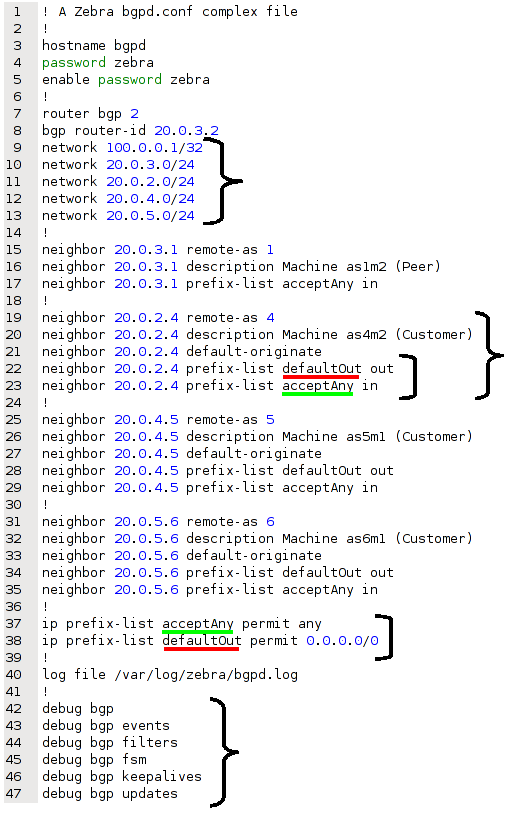
\includegraphics[width=10cm]{images/bgp_conf_schema.png}
	\caption{Una configurazione complessa di BGP.}
	\label{figura:bgp_conf_schema}
\end{figure}

Osservando la struttura del file di configurazione proposto, notiamo subito che vi è una struttura comune che può essere estrapolata e classificata. Senza considerare le righe $1\mapsto8$ che sono riconducibili ad una semplice lista di coppie chiave-valore, soffermiamoci alle righe $9\mapsto13$; qui troviamo le network annunciate dal router in questione e possiamo gia' identificare che tale struttura è una lista con cardinalità 0..n di coppie con chiave ``network'' e con valore uguale all'indirizzo IP più netmask che si vuole annunciare. Già in questo scenario una coppia chiave-valore (usata nella versione $1.0$ di \visualnetkit{}) non può essere utilizzata poiché solitamente le chiavi devono rimanere univoche.

Osserviamo ora le righe $15\mapsto35$ e soffermiamoci in particolare sulle righe $19\mapsto23$. Come descritto nella documentazione di Zebra\cite{ZEBRADOC} un ``peer'' ha la seguente sintassi:
\\
\\
\textbf{neighbor} \textit{peer} \textbf{remote-as} \textit{AS-Number}
\\
\textbf{neighbor} \textit{peer} \textbf{COMMAND}
\\
\\
dove \textbf{COMMAND} è uno dei comandi previsti da Zebra come ad esempio: \emph{description, default-originate, interface, version,} ecc\ldots nonché comandi atti al \emph{Peer Filtering} quali: \emph{discribuite-list, prefix-list, route-map,} ecc\ldots

\begin{figure}[!htb]
	\centering
	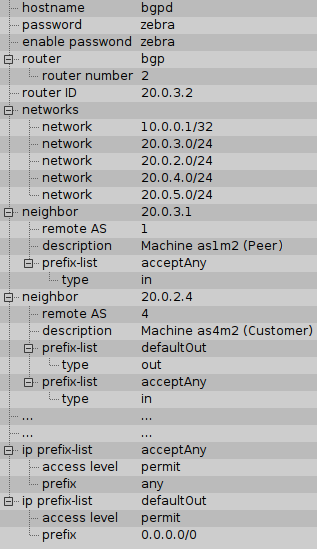
\includegraphics[width=6cm]{images/bgp_conf_tree.png}
	\caption{Configurazione complessa di BGP con struttura gerarchica.}
	\label{figura:bgp_conf_tree}
\end{figure}

Quindi, anche in questo caso è possibile raggruppare le varie definizioni dei ``vicini'' (neighbor) in una struttura gerarchica dove ogni neighbor ha una truttura composta da sotto proprietà, eventualmente con proprietà che si riferiscono a nodi esterni come nel nostro caso \emph{prefix-list} (righa $22-23$). Proprio partendo da queste due righe, possiamo identificare quindi proprietà correlate (simili al concetto di chiavi esterne in uno schema relazionale di basi di dati) a entità esterne; stiamo in definitiva affermando che quella che abbiamo davanti non è nient'altro che una struttura ad albero n-ario che possiede un enorme potere descrittivo, ma allo stesso tempo una struttura complessa da gestire e manipolare. In figura \ref{figura:bgp_conf_tree} viene mostrata la mappatura del file di configurazione in esame (figura \ref{figura:bgp_conf_schema}) in un albero n-ario.

Quella appena mostrata non è che una delle tante possibili interpretazioni di un file di configurazione in una struttura gerarchica. Solitamente ogni file di configurazione (soprattutto nei sistemi \emph{Unix like}) possiede una struttura che è riconducibile ad una con caratteristiche gerarchiche. Proprio verso questa direzione l'evoluzione che \visualnetkit{} ha avuto si è mossa, in particolare tranformando il vecchio modello chiave-valore delle proprietà dei \plugin{}, in uno altamente dinamico (con la possibilità di inserire e/o eliminare proprietà) con struttura annidata.

\subsection{Configurazione avanzata in OSPF}
Ora tenteremo di applicare quanto detto pocanzi ad un altro scenario reale che coinvolge il protocollo OSPF ed il suo file di configurazione. Prendiamo dunque in esame il file di configurazione mostrato in figura \ref{figura:ospf_conf}.

\begin{figure}[!htb]
	\centering
	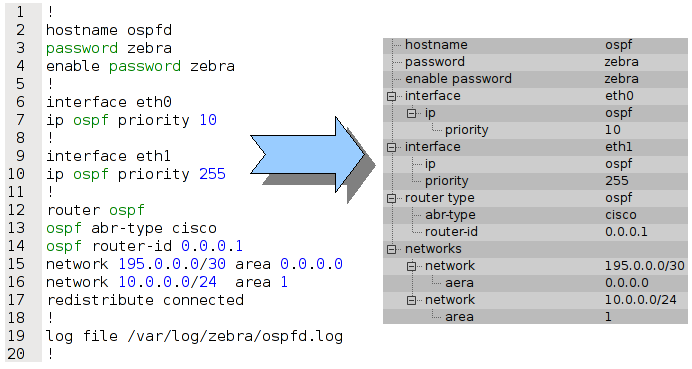
\includegraphics[width=12cm]{images/ospf_conf_schema_tree.png}
	\caption{Configurazione di OSPF e relativa vista gerarchica.}
	\label{figura:ospf_conf}
\end{figure}

Anche in questo caso possiamo procedere nel cercar di trasformare il contenuto del file di configurazione proposto, in una stuttura descritta da un albero n-ario. Iniziamo quindi ad analizzare il testo soffermandoci nelle righe $6\mapsto10$; possimo subito notare come quasta porzione abbia una struttura abbastanza uniforme - come descritto nella documentazione\cite{ZEBRADOC} - che può essere mappata all'interno di una struttura più auto descrittiva e gerarchica (figura \ref{figura:ospf_conf}).

Soffermiamoci ora sulle righe $15-16$ tralasciando le altre. In questo caso possiamo recavare una struttura ben precisa che nella documentazione di Zebra viene presentata nel seguente modo:
\\
\\
\textbf{network} \textit{a.b.c.d/m} \textbf{area} \textit{a.b.c.d}
\\
\textbf{network} \textit{a.b.c.d/m} \textbf{area} <\textit{0-4294967295}>
\\
\\
Naturalmente questi scenari sono soltanto alcuni dei tanti possibili contenuti che si possono trovare all'interno delle varie configurazioni, tuttavia abbiamo appena mostrato che qualunque siano le regole presenti nelle varie impostazioni dei servizi utilizzati, si riesce sempre a ricondurre questi ad una rappresentazione gerarchica talvolta anche complessa.

\section{Requisiti per un Ambiente di Configurazione Avanzata}
Prima di focalizzare gli sforzi nel trasformare il sistema in modo da essere riadattato a quanto detto fin'ora, è preferibile formalizzare i nuovi requisiti - sia quelli funzionali, che non - per avere un quadro complessivo ma charo e non ambiguo su quello che il nuovo sistema dovrà offrire. 

Si è cercato di individuare gli attori principali discutendo con gli \stakeholders{} per avere più punti vi vista. Gli attori individuati sono due:
\begin{itemize}
\item l'utente che utilizza \visualnetkit{}, in particolare uno dei suoi \plugin{};
\item l'utente/sviluppatore che desidera realizzare un \plugin{} dalle caratteristiche avanzate.
\end{itemize}
Sono stati quindi definiti una serie di scenari principali di successo per ciascun caso d'uso semplificato. L'insieme degli scenari ritenuto più importante è presentato in seguito. Si denota con il termine ``end user'' l'utente che utilizza \visualnetkit{}, e con il termine ``plugin developer'' colui che vuole realizzare un \plugin{}.

\begin{flushleft}
\begin{boxedminipage}{\textwidth}

\subsubsection*{Caso d'uso - Inizializzazione dei plugin selezionati}

\textbf{Scopo:} applicazione \visualnetkit{} \\
\textbf{Livello:} user goal \\
\textbf{Attore Primario:} End user \\
\textbf{Parti interessate e interessi:}
\begin{itemize}
\item End user: Desidera un interazione semplice, veloce ed intuitiva con il sistema per raggiungere i propri obiettivi con il minimo sforzo.
\end{itemize}

\textbf{Prerequisiti:} Il sistema deve essere avviato e l'utente deve aver creato un nuovo Lab. \\
\textbf{Goal:} L'utente ha creato un elemento base (una virtual machine, un collision domain o un link) e aver scelto ed inizializzato i \plugin{} che ha selezionato. Il sistema mostra sulla scena grafica l'elemento creato. \\

\textbf{Scenario di successo:}
\begin{enumerate}
\item l'utente seleziona dalla tool bar o dal menu la tipologia dell'elemento che intende aggiungere;
\item l'utente clicca con il mouse - tasto sinistro - un punto della scena grafica e il sistema provvede a mostrare la form per l'inizializzazione dei parametri;
\item l'utente completa la form attivando inoltre i \plugin{} che desidera siano caricati per quel determinato elemento;
\item se l'utente vuole modificare i valori di default dei \plugin{} selezionati, il sistema mostra all'utente una successiva form che offre la possibilità di modificare i vari campi delle property, nonché la possibilità di modificare la struttura delle stesse tramite l'apposito bottone ``actions'';
\item l'utente accetta e il sistema provvede a chiudere la form;
\item il sistema inizializza e aggiorna il suo stato aggiungendo l'elemento selezionato mostrandolo all'utente.
\end{enumerate}

\end{boxedminipage}
\end{flushleft}

\begin{flushleft}
\begin{boxedminipage}{\textwidth}

\subsubsection*{Caso d'uso - Modifica delle proprietà di un elemento}

\textbf{Scopo:} applicazione \visualnetkit{} \\
\textbf{Livello:} user goal \\
\textbf{Attore Primario:} End user \\
\textbf{Parti interessate e interessi:}
\begin{itemize}
\item End user: Desidera un interazione semplice, veloce ed intuitiva con il sistema per raggiungere i propri obiettivi con il minimo sforzo.
\end{itemize}

\textbf{Prerequisiti:} Il sistema deve essere avviato e l'utente deve aver creato un nuovo Lab e deve essere presente almeno un elemento base. \\
\textbf{Goal:} L'utente è riuscito con successo a modificare - contenuto o struttura - una delle proprietà di un elemento selezionato. Il sistema ha provveduto all'acquisizione dei cambiamenti modificando le proprie strutture interne.

\textbf{Scenario di successo:}
\begin{enumerate}
\item l'utente clicca due volte con il mouse - tasto sinistro - un elemento presente nella scena grafica oppure clicca una sola volta un elemento mostrato nell'insieme degli oggetti presenti, selezionandolo;
\item il sistema provvede mostrare le proprietà dell'elemento selezionato nella ``property dock'' catalogate e suddivise in base al loro ruolo: proprietà proprie dell'elemento base e proprietà offerte dai \plugin{} attivi;
\item l'utente modifica il contenuto di una proprietà. Il sistema provvede a validare il valore inserito e a registrare i cambiamenti effettuari eventualmente aggiornando gli elementi grafici;
\item l'utente vuole modificare la struttura delle proprietà di uno dei \plugin{} presenti:
	\begin{enumerate}
	\item l'utente vuole aggiungere una proprietà o sotto-proprietà dopo averne selezionata un'altra. Tramite l'apposito bottone ``actions'' l'utente può inserire altre sotto-proprietà che automaticamente il sistema propone come possibili candidate. Dopo che l'utente ha inserito una nuova proprietà, il sistema registra il cambiamento al suo interno;
	\item l'utente vuole eliminare una proprietà dopo averla selezionata. Tramite il bottone ``actions'' l'utente seleziona ``elimina proprietà'' e il sistema (validando o meno l'operazione) provvede a modificare le proprie strutture interne.
	\end{enumerate}
\end{enumerate}

\end{boxedminipage}
\end{flushleft}
Abbiamo visto i due principali scenari di successo che l'utente finale si dovrebbe aspettare, ora andremo ad analizzare altri scenari di successo che si occupano delle aspettative dell'utente (\plugin{} developer) che vuole creare un plugin offri la possibilità di impostare configurazioni avanzate per il servizio che descrive.

\begin{flushleft}
\begin{boxedminipage}{\textwidth}

\subsubsection*{Caso d'uso - Creazione di \plugin{} avanzati}

\textbf{Scopo:} \plugin{} per \visualnetkit{} \\
\textbf{Livello:} subfunction \\
\textbf{Attore Primario:} plugin developer \\
\textbf{Parti interessate e interessi:}
\begin{itemize}
\item Plugin developer: Si aspetta di riuscir a creare il proprio \plugin{} che dovrà contenere una struttura flessibile da poter descrivere la maggior parte delle configurazioni avanzate di un certo servizio offerto dal \plugin{} stesso.
\end{itemize}

\textbf{Goal:} Lo sviluppatore realizza un \plugin{} per un determinato servizio che al suo interno possiede flessibilità e alta adattabilità in modo da offrire anche configurazioni complesse.

\textbf{Scenario di successo:}
\begin{enumerate}
\item lo sviluppatore costruire il file di configurazione per il suo \plugin{} descrivendo in modo dettagliato la struttura delle proprietà;
\item lo sviluppatore crea il proprio \plugin{} che offrirà agli utenti finali la possibilità di una particolare estensione dell'elemento base su cui si basa il \plugin{};
\item il sistema provvederà a caricare il plugin durante l'avvio e ad offrire all'utente finale la possibilità di selezionarlo.
\end{enumerate}

\end{boxedminipage}
\end{flushleft}

In figura \ref{figura:uc1} viene proposto il diagramma completo dei casi d'uso e l'interazione tra essi.

\begin{figure}[!htb]
	\centering
	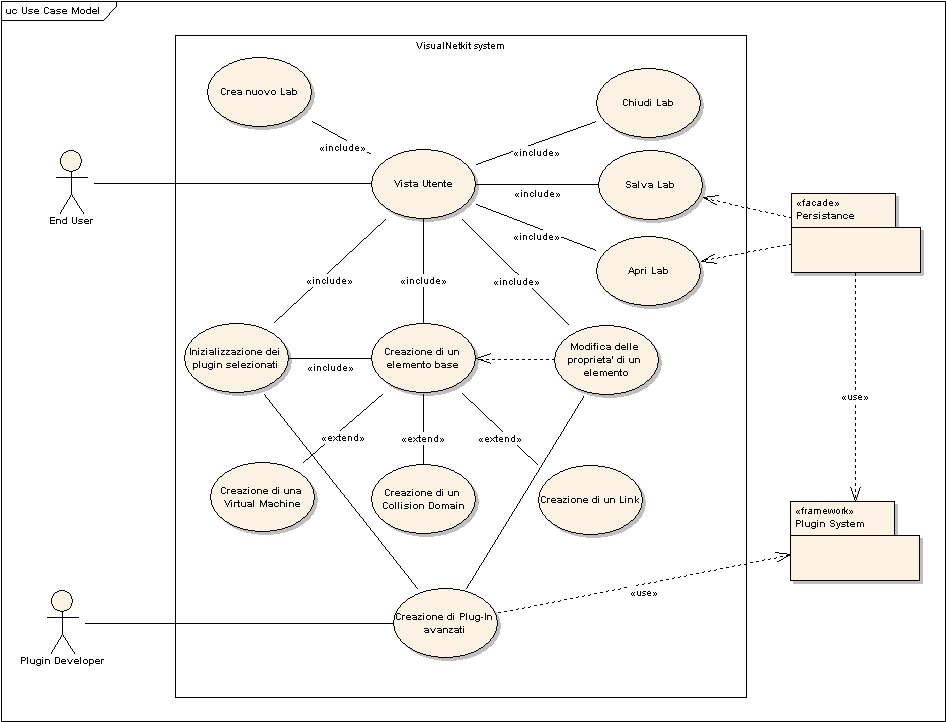
\includegraphics[width=12cm]{images/UseCaseModel.png}
	\caption{Diagramma dei casi d'uso principali in \visualnetkit{}.}
	\label{figura:uc1}
\end{figure}

\subsubsection{L'impatto sul sistema}
Analizziamo ora in dettaglio quale sarà l'impatto sul sistema che prevede property unicamente descritte da una lista di coppie chiave-valore. Stiamo di fatto introducendo un cambiamento abbastanza radicale che andrà a coinvolcege da una parte il core di \visualnetkit{} e dall'altra il framework che supporta l'architettura modulare. Scendendo nei particolari ci si dovrà muovere con una strategia \bu{} effettuando un restyle del \plugin{} framework introducendo nuove funzionalità. Queste ultime interaggiranno con i moduli per interrogare le loro proprietà\footnote{Si ricorda che le proprietà saranno contenute in strutture ad alberi n-ari, non facilmente gestibili.} e per validare ed interpellare il loro file di configurazione \xml{}.

Fatto ciò, si salirà sulla scala gerarchica fino ad arrivare a rimodellare la GUI che sarà dotata di una nuova property dock. Anche il core stesso dell'applicazione dovrà essere rivisto; i vari handler che raccolgono le modifiche effettuate dall'utente all'intnerno delle proprietà, andranno migliorati e correlati tra loro. In tutto questo giocherà un ruolo fondamentale il potente framework \qt{}, basato pesantemente sul pattern architetturale \emph{MVC}\cite{QTDOCMVC}.

\section{Analisi Architetturale}
In questa sezione raccoglieremo tutti i requisiti descritti precedentemente e, rispettando la tassonomia dell'attuale sistema, cercheremo di formalizzare le modifiche che si dovranno poi riflettere su \visualnetkit{}. Una prima fase di analisi è stata spesa per carpire adeguatamente il tipo di supporto offerto da \qt{}, in particolare i concetti che stanno dietro il sistema \emph{Model/View}.

\subsubsection*{L'architettura Model/View in \qt{}}
Model-View-Controller (MVC) è un pattern originario da \emph{Smaltalk} che è spesso usato quando si ha a che fare con incerfacce utente. \qt{} separa le varie classi all'interno di tre gruppi: models, views e delegates. Ognuno di questi componenti sono definiti da una classe astratta comune che offre implementazioni di default di uso generico.

\begin{figure}[!htb]
	\centering
	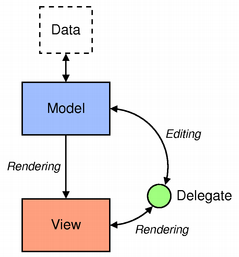
\includegraphics[width=6cm]{images/modelview-overview.png}
	\caption{MVC all'interno di \qt{}$4$.}
	\label{figura:qt_mvc}
\end{figure}

Tutti i modelli sono basati sulla classe \emph{QAbstractItemModel}. Questa definisce un interfaccia che viene usata dalla vista (View) attraverso il delegato, per accedere ai dati. I dati stessi non sono presenti nel modello, ma vengono immagazzinati in strutture separate che possono essere classi, files, database o altri tipi di componenti.

Le viste invece implentano la parte visiva dei dati, presentata all'utente finale. \qt{} offre tre tipologie di viste utilizzate a seconda dei casi: Tabelle, Liste o Alberi. In particolare ogni vista renderizza le informazieni (tramite il delegato) presenti nelle strutture dati gestite dal modello, e questo offre la possibilità che ogni modello possa essere visualizzato all'interno di viste differenti\footnote{Si pensi a dati anagrafici che devono essere mostrati in più tipologie di grafici; grafici a torta, a barre, istogrammi, ecc\ldots}.

I delegati sono elementi di estrema importanza all'interno del framework. Questi fungono da livello di indirezione tra la vista e il modello ed offrono supporto alla renderizzazione dei dati. È infatti possibile reimplementare la classe astratta che descrive tutti i delegati (\emph{QAbstractItemDelegate}) per poter ad esempio inserire diversi widget di input nei campi mostrati in una tabella, come mostrato in figura \ref{figura:qt_delegate}.

\begin{figure}[!htb]
	\centering
	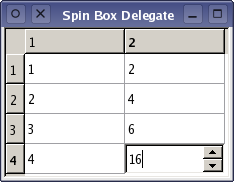
\includegraphics[width=6cm]{images/spinboxdelegate-example.png}
	\caption{Un esempio di ``delegate'' in \qt{}$4$.}
	\label{figura:qt_delegate}
\end{figure}

\subsubsection*{Utilizzo di MVC nel nuovo property system}
Quanto appena descritto ha giocato un ruolo fondamentale nel comprendere il metodo di effettuare le modifiche alle proprietà nel miglior modo, utilizzando al meglio gli strumenti offerti da \qt{}. Come primo test si è partiti con un prototipo di property editor sul quale effettuare i vari esperimenti, cercando di mantenere il codice pulito per il riuso.
Questa fase si affronta solitamente per andare in contro ai problemi, affrontarli e risolverli al meglio. Il modello di MVC che \qt{} propone è stato sfruttato in tutti i suoi dettagli tranne che per i delegati in quanto, per gli scopi prefissati, non erano previste tipizzazioni nei campi valori delle proprietà.

Si è quindi partiti nel creare una struttura ad albero n-ario, passando alla creazione del modello, ed in fine gli sforzi si sono concerntrati sulla vista e sull'interazione tra essa e il modello stesso, ponendo particolare attenzione all'accoppiamento e alla coesione degli oggetti.

Durante la modellazione è stato deciso di accentrare il controllo su di un entità astratta che fosse stata in stretto contatto con i dati e che raccogliesse le richieste di cambiamento. Il problema si è presentato perchè il property editor è utilizzato non solo dagli elementi base di \visualnetkit{}, ma anche ad altri componenti quali Aree grafiche e proprietà stesse del laboratorio. Da qui la necessità di generalizzare il concetto di ``property handler'' che potesse essere abbastanza generale da essere esteso dai vari controllers concreti. Di questo ci occuperemo più in dettaglio nella successiva sezione.

\subsection{\plugin{} per la Configurazione Avanzata}
In questa parte ci occuperemo ad analizzare quanto detto poc'anzi. Osserviamo quindi la figura \ref{figura:properties_uml1}.

\begin{figure}[!htb]
	\centering
	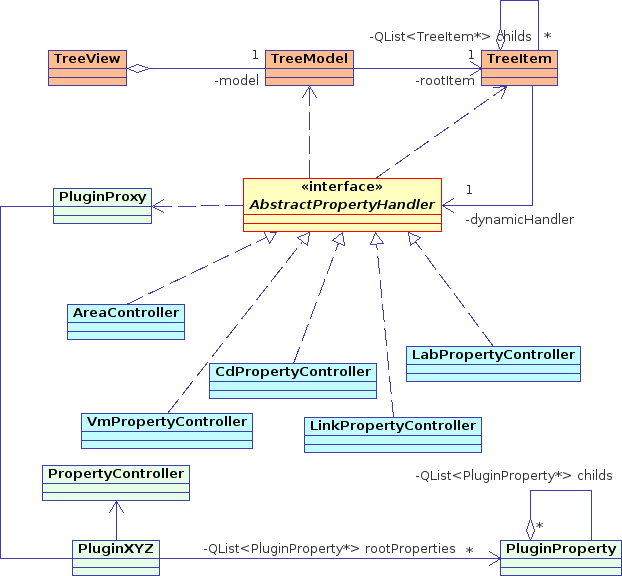
\includegraphics[width=10cm]{images/properties_uml1.png}
	\caption{Diagramma delle classi del nuovo sistema.}
	\label{figura:properties_uml1}
\end{figure}

Notiamo subito la presenza di una generalizzazione per quanto riguarda il property handler, come accennato precedentemente. Tale interfaccia (in \cpp{} è chiamata una ``pure abstract class'') offre le seguenti funzioni:
\begin{description}
\item[getComposedModel()]questa funzione indica che ogni classe che la estende deve necessariamente fornire un model appropriamente costruito che verrà poi collegato alla vista. Il model viene creato ricavando le informazioni dall'elemento base e dalle properties offerte dai vari plugins che aggrega. Ogni ``tree item'' possiede quindi il riferimento al suo creatore che è anche l'oggetto che riceve le richieste di cambiamento;

\item[getInitMolel()]questa funzione viene usata dalle sotto classi che adempiono il ruolo di property controllers per gli elementi base\footnote{Ricordiamo che per ``elemento base'' in \visualnetkit{} si intendono Virtual Machines, Collision Domains e Links.}, fornendo un modello simile al precedente ma che contiene solamente i dati dei plugins selezionati;

\item[saveChangedProperty()]viene utilizzata per il salvataggio dei cambiamenti effettuati in una determinata proprerty.

\item[getPluginFromCurrentElement()]questa funzione è puramente di convenienza e viene usata di rado;

\item[removePluginProperty()]viene utilizzata per inoltrare la richiesta di eliminazione di una property di un plugin. Il controllo di consistenza viene effettuato dal plugin stesso;

\item[addPluginProperty()]come sopra, ma utilizzata per inserire una property (o sotto property) in un plugin.
\end{description}

Arriviamo quindi ad avere un forte incremento di flessibilità ed estensibilità grazie all'aggunta di properties dei plugins non più statiche, ma dinamiche con struttura anche annidata (figura \ref{figura:property_editor_paragone}).

\begin{figure}[!htb]
	\centering
	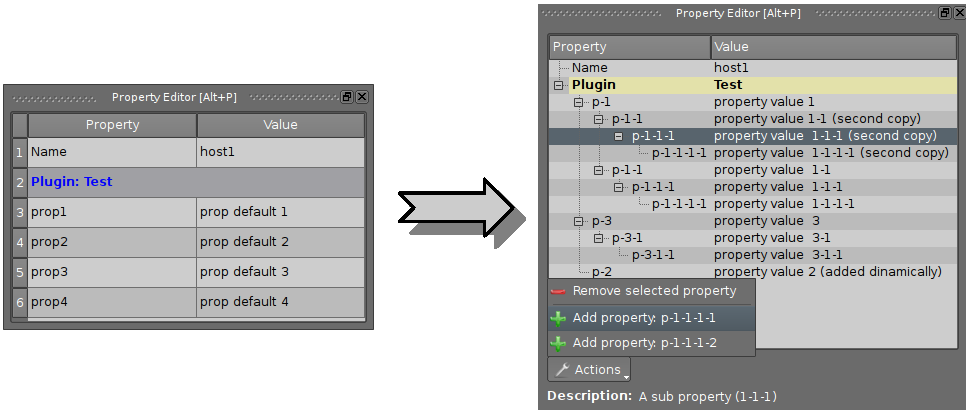
\includegraphics[width=12cm]{images/property_editors_paragone.png}
	\caption{Paragone tra il vecchio ed il nuovo property editor.}
	\label{figura:property_editor_paragone}
\end{figure}


\subsection{Metodologie di sviluppo adottate}
Al fine di rendere la progettazione più corretta e la fase di implementazione meno rischiosa si è cercato di cogliere gli aspetti qualificanti di metodologie di sviluppo quali \textit{XP}, \textit{FDD} e le più note metodologie di sviluppo iterativo come \textit{UP} (\emph{Unified Process}).\\
Seguendo le linee guida dettate da \textit{UP}, si è optato per la definizione di cicli di sviluppo scanditi dal rilascio di prototipi funzionanti del progetto e dalla loro presentazione e discussione, così da avere una valutazione dell'avanzamento del progetto e una buona gestione dei fattori di rischio. Ogni ciclo è stato suddiviso in tre fasi: \textit{inception phase}, \textit{elaboration phase} e \textit{construction phase}.
Scopo principale della fase iniziale è stato quello di delineare, nel modo più accurato possibile, il caso di interesse e identificare gli elementi importanti affinché esso conduca al completamento delle funzionalità desiderate.

Nel primo ciclo di analisi e progettazione, questa fase è stata supportata da strumenti quali un modello dei casi d'uso sufficientemente dettagliato da definire i principali obiettivi del progetto, una pianificazione del progetto e delle prime fasi evolutive, una valutazione dei rischi ed una definizione primaria dei requisiti.
La fase di elaborazione ha contribuito a definire la struttura complessiva del sistema. Questa fase ha compreso l'analisi di dominio ed un prima fase di progettazione dell'architettura a cui si è affiancato lo studio per la rappresentazione del modello logico.

Al termine di queste due è seguita una fase conclusiva di implementazione e rilascio di un prototipo e sottoversioni dell'architettura, capaci di mostrare il completamento dei casi d'uso principali e delle funzionalità introdotte nelle fasi precedenti.

A dispetto delle linee guida proposte dalla metodologia UP, le quali prevedono una quarta \textit{fase di transizione} in cui vengono condotte le attività di training e il \textit{beta testing}\footnote{Il beta testing (o beta-verifica) è una fase di prova e collaudo di un software non ancora pubblicato, con lo scopo di trovare eventuali errori (bug). Questa operazione può essere svolta da professionisti pagati, oppure, molto spesso, da semplici amatori (chiamati beta-testers).} del sistema a scopo di verifica e validazione, ogni fase è stata arricchita da piccole iterazioni di analisi e test, limitando considerevolmente l'overhead complessivo.

La metodologia XP è stata abbracciata in particolare nella verifica continua del progetto, la frequente reingegnerizzazione del software e la libertà di seguire o meno le fasi di sviluppo prefissate, il tutto a beneficio del progetto. Nelle fasi finali di sviluppo, per il raffinamento e perfezionamento delle funzionalità accessorie, si è optato per un tipo di sviluppo orientato verso FDD.
\textit{FDD} o \textit{Feature Driven Development}, anch'essa parte dell'\textit{Agile Manifesto}, cerca di spingere XP verso un'estrema flessibilità, eliminando interamente la fase classica di progettazione, volgendo il pieno interesse verso le fasi di \textit{definizione di una lista di funzionalità} e di uno \textit{sviluppo per funzionalità}, impostate in maniera tale da ottenere una frammentazione (una granularità) dall'alto verso il basso in modo da essere prodotte in brevi iterazioni.
